\chapter{深度优先搜索}


\section{Palindrome Partitioning} %%%%%%%%%%%%%%%%%%%%%%%%%%%%%%
\label{sec:palindrome-partitioning}


\subsubsection{描述}
Given a string s, partition s such that every substring of the partition is a palindrome.

Return all possible palindrome partitioning of s.

For example, given \code{s = "aab"},
Return
\begin{Code}
  [
    ["aa","b"],
    ["a","a","b"]
  ]
\end{Code}


\subsubsection{分析}
在每一步都可以判断中间结果是否为合法结果,用回溯法。

一个长度为n的字符串,有n+1个地方可以砍断,每个地方可断可不断,因此复杂度为$O(2^{n+1})$


\subsubsection{代码}
\begin{Code}
//LeetCode, Palindrome Partitioning
class Solution {
public:
    vector<vector<string>> partition(string s) {
        vector<vector<string>> result;
        vector<string> output;  // 一个partition方案
        DFS(s, 0, output, result);
        return result;
    }
    // 搜索必须以s[start]开头的partition方案
    // 如果一个字符串长度为n,则可以插入n+1个隔板,复制度为O(2^{n+1})
    void DFS(string &s, int start, vector<string>& output,
            vector<vector<string>> &result) {
        if (start == s.size()) {
            result.push_back(output);
            return;
        }
        for (int i = start; i < s.size(); i++) {
            if (isPalindrome(s, start, i)) { // 从i位置砍一刀
                output.push_back(s.substr(start, i - start + 1));
                DFS(s, i + 1, output, result);  // 继续往下砍
                output.pop_back(); // 撤销上一个push_back的砍
            }
        }
    }
    bool isPalindrome(string &s, int start, int end) {
        while (start < end) {
            if (s[start] != s[end]) return false;
            start++;
            end--;
        }
        return true;
    }
};
\end{Code}


\subsubsection{相关题目}

\begindot
\item Palindrome Partitioning II,见 \S \ref{sec:palindrome-partitioning-ii}
\myenddot


\section{Unique Paths} %%%%%%%%%%%%%%%%%%%%%%%%%%%%%%
\label{sec:unique-paths}


\subsubsection{描述}
A robot is located at the top-left corner of a $m \times n$ grid (marked 'Start' in the diagram below).

The robot can only move either down or right at any point in time. The robot is trying to reach the bottom-right corner of the grid (marked 'Finish' in the diagram below).

How many possible unique paths are there?

\begin{center}
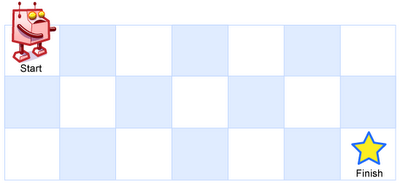
\includegraphics[width=300pt]{robot-maze.png}\\
\figcaption{Above is a $3 \times 7$ grid. How many possible unique paths are there?}\label{fig:unique-paths}
\end{center}

\textbf{Note}: $m$ and $n$ will be at most 100.


\subsection{深搜}
深搜,小集合可以过,大集合会超时

\subsubsection{代码}
\begin{Code}
// LeetCode, Unique Paths
// 深搜,小集合可以过,大集合会超时
class Solution {
public:
    int uniquePaths(int m, int n) {
        this->m = m;
        this->n = n;
        return uniquePathsRecursive(m, n);
    }
private:
    int m, n;

    int uniquePathsRecursive(int x, int y) {
        if (x < 1 or x > m) return 0; // 数据非法
        if (y < 1 or y > n) return 0;

        if (x == 1 and y == 1) return 1; // 终止条件

        return uniquePathsRecursive(x - 1, y) + uniquePathsRecursive(x, y - 1);
    }
};
\end{Code}


\subsection{备忘录法}
给前面的深搜,加个缓存,就可以过大集合了。即备忘录法。

\subsubsection{代码}
\begin{Code}
// LeetCode, Unique Paths
// 深搜 + 缓存,即备忘录法
class Solution {
public:
    int uniquePaths(int m, int n) {
        this->m = m;
        this->n = n;
        // 0行和0列未使用
        this->f = vector<vector<int> >(m + 1, vector<int>(n + 1, 0));
        return cachedUniquePathsRecursive(m, n);
    }
private:
    int m, n;  // 全局只读数据
    vector<vector<int> > f;  // 缓存

    int uniquePathsRecursive(int x, int y) {
        if (x < 1 or x > m) return 0; // 数据非法,终止条件
        if (y < 1 or y > n) return 0;

        if (x == 1 and y == 1) return 1; // 回到起点,收敛条件

        return cachedUniquePathsRecursive(x - 1, y) +
                cachedUniquePathsRecursive(x, y - 1);
    }

    int cachedUniquePathsRecursive(int x, int y) {
        if (f[x][y] > 0) return f[x][y];
        else return f[x][y] = uniquePathsRecursive(x, y);
    }
};
\end{Code}


\subsection{动规}
既然可以用备忘录法自顶向下解决,也一定可以用动规自底向上解决。

设状态为\fn{f[i][j]},表示从起点$(1,1)$到达$(i,j)$的路线条数,则状态转移方程为:
\begin{Code}
f[i][j]=f[i-1][j]+f[i][j-1]
\end{Code}


\subsubsection{代码}
\begin{Code}
// LeetCode, Unique Paths
// 动规,滚动数组
class Solution {
public:
    int uniquePaths(int m, int n) {
        vector<int> f(n, 0);
        f[0] = 1;
        for (int i = 0; i < m; i++) {
            for (int j = 1; j < n; j++) {
                // 左边的f[j],表示更新后的f[j],与公式中的f[i[[j]对应
                // 右边的f[j],表示老的f[j],与公式中的f[i-1][j]对应
                f[j] = f[j - 1] + f[j];
            }
        }
        return f[n - 1];
    }
};
\end{Code}


\subsection{数学公式}
一个$m$行,$n$列的矩阵,机器人从左上走到右下总共需要的步数是$m+n-2$,其中向下走的步数是$m-1$,因此问题变成了在$m+n-2$个操作中,选择$m–1$个时间点向下走,选择方式有多少种。即 $C_{m+n-2}^{m-1}$ 。

\subsubsection{代码}
\begin{Code}
// LeetCode, Unique Paths
// 数学公式
class Solution {
public:
    typedef long long int64_t;
    // 求阶乘, n!/(start-1)!,即 n*(n-1)...start,要求 n >= 1
    static int64_t factor(int n, int start = 1) {
        int64_t  ret = 1;
        for(int i = start; i <= n; ++i)
            ret *= i;
        return ret;
    }
    // 求组合数 C_n^k
    static int64_t combination(int n, int k) {
        // 常数优化
        if (k == 0) return 1;
        if (k == 1) return n;

        int64_t ret = factor(n, k+1);
        ret /= factor(n - k);
        return ret;
    }

    int uniquePaths(int m, int n) {
        // max 可以防止n和k差距过大,从而防止combination()溢出
        return combination(m+n-2, max(m-1, n-1));
    }
};
\end{Code}


\subsubsection{相关题目}
\begindot
\item Unique Paths II,见 \S \ref{sec:unique-paths-ii}
\myenddot


\section{Unique Paths II} %%%%%%%%%%%%%%%%%%%%%%%%%%%%%%
\label{sec:unique-paths-ii}


\subsubsection{描述}
Follow up for "Unique Paths":

Now consider if some obstacles are added to the grids. How many unique paths would there be?

An obstacle and empty space is marked as 1 and 0 respectively in the grid.

For example,

There is one obstacle in the middle of a $3 \times 3$ grid as illustrated below.
\begin{Code}
[
  [0,0,0],
  [0,1,0],
  [0,0,0]
]
\end{Code}

The total number of unique paths is 2.

Note: $m$ and $n$ will be at most 100.


\subsection{备忘录法}
在上一题的基础上改一下即可。相比动规,简单得多。

\subsubsection{代码}
\begin{Code}
// LeetCode, Unique Paths II
// 深搜 + 缓存,即备忘录法
class Solution {
public:
    int uniquePathsWithObstacles(vector<vector<int> > &obstacleGrid) {
        const int m = obstacleGrid.size();
        const int n = obstacleGrid[0].size();
        // 0行和0列未使用
        this->f = vector<vector<int> >(m + 1, vector<int>(n + 1, 0));
        return cachedUniquePathsRecursive(obstacleGrid, m, n);
    }
private:
    vector<vector<int> > f;  // 缓存

    int uniquePathsRecursive(const vector<vector<int> > &obstacleGrid,
            int x, int y) {
        if (x < 1 or x > obstacleGrid.size()) return 0; // 数据非法,终止条件
        if (y < 1 or y > obstacleGrid[0].size()) return 0;

        // (x,y)是障碍
        if (obstacleGrid[x-1][y-1]) return 0;

        if (x == 1 and y == 1) return 1; // 回到起点,收敛条件

        return cachedUniquePathsRecursive(obstacleGrid, x - 1, y) +
                cachedUniquePathsRecursive(obstacleGrid, x, y - 1);
    }

    int cachedUniquePathsRecursive(const vector<vector<int> > &obstacleGrid,
            int x, int y) {
        if (f[x][y] > 0) return f[x][y];
        else return f[x][y] = uniquePathsRecursive(obstacleGrid, x, y);
    }
};
\end{Code}


\subsection{动规}
与上一题类似,但要特别注意第一列的障碍。在上一题中,第一列全部是1,但是在这一题中不同,第一列如果某一行有障碍物,那么后面的行应该为0。


\subsubsection{代码}
\begin{Code}
// LeetCode, Unique Paths II
// 动规,滚动数组
class Solution {
public:
    int uniquePathsWithObstacles(vector<vector<int> > &obstacleGrid) {
        const int m = obstacleGrid.size();
        const int n = obstacleGrid[0].size();
        if (obstacleGrid[0][0] || obstacleGrid[m-1][n-1]) return 0;

        vector<int> f(n, 0);

        // 寻找第一列的第一个障碍在哪一行
        int first_col_obstacle = INT_MAX;
        for (int i = 0; i < m; i++) {
            if (obstacleGrid[i][0]) {
                first_col_obstacle = i;
                break;
            }
        }

        for (int i = 0; i < m; i++) {
            // 第一列如果某一行有障碍物,那么后面的行应该为0。
            if(i >= first_col_obstacle) f[0] = 0;
            else f[0] = 1;
            for (int j = 1; j < n; j++) {
                if (!obstacleGrid[i][j]) {
                    // 左边的f[j],表示更新后的f[j],与公式中的f[i[[j]对应
                    // 右边的f[j],表示老的f[j],与公式中的f[i-1][j]对应
                    f[j] = f[j - 1] + f[j];
                } else {
                    f[j] = 0;
                }
            }
        }
        return f[n - 1];
    }
};
\end{Code}


\subsubsection{相关题目}
\begindot
\item Unique Paths,见 \S \ref{sec:unique-paths}
\myenddot


\section{N-Queens} %%%%%%%%%%%%%%%%%%%%%%%%%%%%%%
\label{sec:n-queens}


\subsubsection{描述}
The \emph{n-queens puzzle} is the problem of placing n queens on an $n \times n$ chessboard such that no two queens attack each other.

\begin{center}
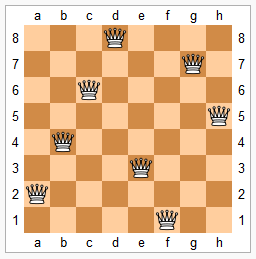
\includegraphics{8-queens.png}\\
\figcaption{Eight Queens}\label{fig:8-queens}
\end{center}

Given an integer $n$, return all distinct solutions to the n-queens puzzle.

Each solution contains a distinct board configuration of the n-queens' placement, where \fn{'Q'} and \fn{'.'} both indicate a queen and an empty space respectively.

For example,
There exist two distinct solutions to the 4-queens puzzle:
\begin{Code}
[
 [".Q..",  // Solution 1
  "...Q",
  "Q...",
  "..Q."],

 ["..Q.",  // Solution 2
  "Q...",
  "...Q",
  ".Q.."]
]
\end{Code}


\subsubsection{分析}
经典的深搜题。

\subsubsection{代码}
\begin{Code}
// LeetCode, N-Queens
// 深搜+剪枝
class Solution {
public:
    vector<vector<string> > solveNQueens(int n) {
        this->columns = vector<int>(n, 0);
        this->principal_diagonals = vector<int>(2 * n, 0);
        this->counter_diagonals = vector<int>(2 * n, 0);

        vector<vector<string> > result;
        vector<int> C(n, 0);  // C[i]表示第i行皇后所在的列编号
        solveNQueens(0, C, result);
        return result;
    }
private:
    // 这三个变量用于剪枝
    vector<int> columns;  // 表示已经放置的皇后占据了哪些列
    vector<int> principal_diagonals;  // 占据了哪些主对角线
    vector<int> counter_diagonals;  // 占据了哪些副对角线

    void solveNQueens(int row, vector<int> &C,
            vector<vector<string> > &result) {
        const int N = C.size();
        if (row == N) { // 终止条件,也是收敛条件,意味着找到了一个可行解
            vector<string> solution;
            for (int i = 0; i < N; ++i) {
                string s(N, '.');
                for (int j = 0; j < N; ++j) {
                    if (j == C[i]) s[j] = 'Q';
                }
                solution.push_back(s);
            }
            result.push_back(solution);
            return;
        }

        for (int j = 0; j < N; ++j) {  // 扩展状态,一列一列的试
            const bool ok = columns[j] == 0 &&
                    principal_diagonals[row + j] == 0
                    && counter_diagonals[row - j + N] == 0;
            if (ok) {  // 剪枝:如果合法,继续递归
                // 执行扩展动作
                C[row] = j;
                columns[j] = principal_diagonals[row + j] =
                        counter_diagonals[row - j + N] = 1;
                solveNQueens(row + 1, C, result);
                // 撤销动作
                // C[row] = 0;
                columns[j] = principal_diagonals[row + j] =
                        counter_diagonals[row - j + N] = 0;
            }
        }
    }
};
\end{Code}


\subsubsection{相关题目}
\begindot
\item N-Queens II,见 \S \ref{sec:n-queens-ii}
\myenddot


\section{N-Queens II} %%%%%%%%%%%%%%%%%%%%%%%%%%%%%%
\label{sec:n-queens-ii}


\subsubsection{描述}
Follow up for N-Queens problem.

Now, instead outputting board configurations, return the total number of distinct solutions.


\subsubsection{分析}
只需要输出解的个数,不需要输出所有解,代码要比上一题简化很多。设一个全局计数器,每找到一个解就增1。


\subsubsection{代码}
\begin{Code}
// LeetCode, N-Queens II
// 深搜+剪枝
class Solution {
public:
    int totalNQueens(int n) {
        this->count = 0;
        this->columns = vector<int>(n, 0);
        this->principal_diagonals = vector<int>(2 * n, 0);
        this->counter_diagonals = vector<int>(2 * n, 0);

        vector<vector<string> > result;
        vector<int> C(n, 0);  // C[i]表示第i行皇后所在的列编号
        solveNQueens(0, C, result);
        return this->count;
    }
private:
    int count; // 解的个数
    // 这三个变量用于剪枝
    vector<int> columns;  // 表示已经放置的皇后占据了哪些列
    vector<int> principal_diagonals;  // 占据了哪些主对角线
    vector<int> counter_diagonals;  // 占据了哪些副对角线

    void solveNQueens(int row, vector<int> &C,
            vector<vector<string> > &result) {
        const int N = C.size();
        if (row == N) { // 终止条件,也是收敛条件,意味着找到了一个可行解
            this->count++;
            return;
        }

        for (int j = 0; j < N; ++j) {  // 扩展状态,一列一列的试
            const bool ok = columns[j] == 0 &&
                    principal_diagonals[row + j] == 0
                    && counter_diagonals[row - j + N] == 0;
            if (ok) {  // 剪枝:如果合法,继续递归
                // 执行扩展动作
                C[row] = j;
                columns[j] = principal_diagonals[row + j] =
                        counter_diagonals[row - j + N] = 1;
                solveNQueens(row + 1, C, result);
                // 撤销动作
                // C[row] = 0;
                columns[j] = principal_diagonals[row + j] =
                        counter_diagonals[row - j + N] = 0;
            }
        }
    }
};
\end{Code}


\subsubsection{相关题目}
\begindot
\item N-Queens,见 \S \ref{sec:n-queens}
\myenddot


\section{Restore IP Addresses} %%%%%%%%%%%%%%%%%%%%%%%%%%%%%%
\label{sec:restore-ip-addresses}


\subsubsection{描述}
Given a string containing only digits, restore it by returning all possible valid IP address combinations.

For example:
Given \code{"25525511135"},

return \code{["255.255.11.135", "255.255.111.35"]}. (Order does not matter)


\subsubsection{分析}
必须要走到底部才能判断解是否合法,深搜。


\subsubsection{代码}
\begin{Code}
// LeetCode, Restore IP Addresses
class Solution {
public:
    vector<string> restoreIpAddresses(string s) {
        vector<string> result;
        string ip; // 存放中间结果
        dfs(s, 0, 0, ip, result);
        return result;
    }

    /**
     * @brief 解析字符串
     * @param[in] s 字符串,输入数据
     * @param[in] startIndex 从s的哪里开始
     * @param[in] step 当前步骤编号,从0开始编号,取值为0,1,2,3,4表示结束了
     * @param[out] intermediate 当前解析出来的中间结果
     * @param[out] result 存放所有可能的IP地址
     * @return 无
     */
    void dfs(string s, int start, int step, string ip,
            vector<string> &result) {
        if (s.size() - start > (4 - step) * 3)
            return;  // 非法结果,剪枝
        if (s.size() - start < (4 - step))
            return;  // 非法结果,剪枝

        if (start == s.size() && step == 4) {  // 找到一个合法解
            ip.resize(ip.size() - 1);
            result.push_back(ip);
            return;
        }

        int num = 0;
        for (int i = start; i < start + 3; i++) {
            num = num * 10 + (s[i] - '0');

            if (num <= 255) {  // 当前结点合法,则继续往下递归
                ip += s[i];
                dfs(s, i + 1, step + 1, ip + '.', result);
            }
            if (num == 0) break;  // 不允许前缀0,但允许单个0
        }
    }
};
\end{Code}


\subsubsection{相关题目}
\begindot
\item 无
\myenddot


\section{Combination Sum} %%%%%%%%%%%%%%%%%%%%%%%%%%%%%%
\label{sec:combination-sum}


\subsubsection{描述}
Given a set of candidate numbers ($C$) and a target number ($T$), find all unique combinations in $C$ where the candidate numbers sums to $T$.

The same repeated number may be chosen from $C$ \emph{unlimited} number of times.

Note:
\begindot
\item All numbers (including target) will be positive integers.
\item Elements in a combination ($a_1, a_2, ..., a_k$) must be in non-descending order. (ie, $a_1 > a_2 > ... > a_k$).
\item The solution set must not contain duplicate combinations.
\myenddot

For example, given candidate set \fn{2,3,6,7} and target \fn{7}, 
A solution set is: 
\begin{Code}
[7] 
[2, 2, 3] 
\end{Code}


\subsubsection{分析}
无


\subsubsection{代码}
\begin{Code}
// LeetCode, Combination Sum
class Solution {
public:
    vector<vector<int> > combinationSum(vector<int> &nums, int target) {
        std::sort(nums.begin(), nums.end());
        vector<vector<int> > result; // 最终结果
        vector<int> intermediate; // 中间结果
        dfs(nums, target, 0, intermediate, result);
        return result;
    }

private:
    void dfs(vector<int>& nums, int gap, int level, vector<int>& intermediate,
            vector<vector<int> > &result) {
        if (gap == 0) {  // 找到一个合法解
            result.push_back(intermediate);
            return;
        }
        for (size_t i = level; i < nums.size(); i++) { // 扩展状态
            if (gap < nums[i]) return; // 剪枝

            intermediate.push_back(nums[i]); // 执行扩展动作
            dfs(nums, gap - nums[i], i, intermediate, result);
            intermediate.pop_back();  // 撤销动作
        }
    }
};
\end{Code}


\subsubsection{相关题目}
\begindot
\item Combination Sum II ,见 \S \ref{sec:combination-sum-ii}
\myenddot


\section{Combination Sum II} %%%%%%%%%%%%%%%%%%%%%%%%%%%%%%
\label{sec:combination-sum-ii}


\subsubsection{描述}
Given a set of candidate numbers ($C$) and a target number ($T$), find all unique combinations in $C$ where the candidate numbers sums to $T$.

The same repeated number may be chosen from $C$ \emph{once} number of times.

Note:
\begindot
\item All numbers (including target) will be positive integers.
\item Elements in a combination ($a_1, a_2, ..., a_k$) must be in non-descending order. (ie, $a_1 > a_2 > ... > a_k$).
\item The solution set must not contain duplicate combinations.
\myenddot

For example, given candidate set \fn{10,1,2,7,6,1,5} and target \fn{8}, 
A solution set is: 
\begin{Code}
[1, 7] 
[1, 2, 5] 
[2, 6] 
[1, 1, 6]
\end{Code}


\subsubsection{分析}
无


\subsubsection{代码}
\begin{Code}
// LeetCode, Combination Sum II
class Solution {
public:
    vector<vector<int> > combinationSum2(vector<int> &nums, int target) {
        std::sort(nums.begin(), nums.end()); // 跟第 50 行配合,
                                             // 确保每个元素最多只用一次
        vector<vector<int> > result;
        vector<int> intermediate;
        dfs(nums, target, 0, intermediate, result);
        return result;
    }
private:
    // 使用nums[index, nums.size())之间的元素,能找到的所有可行解
    static void dfs(vector<int> &nums, int gap, int index,
            vector<int> &intermediate, vector<vector<int> > &result) {
        if (gap == 0) {  //  找到一个合法解
            result.push_back(intermediate);
            return;
        }

        int previous = -1;
        for (size_t i = index; i < nums.size(); i++) {
            // 如果上一轮循环没有选nums[i],则本次循环就不能再选nums[i],
            // 确保nums[i]最多只用一次
            if (previous == nums[i]) continue;

            if (gap < nums[i]) return;  // 剪枝

            previous = nums[i];

            intermediate.push_back(nums[i]);
            dfs(nums, gap - nums[i], i + 1, intermediate, result);
            intermediate.pop_back();  // 恢复环境
        }
    }
};
\end{Code}


\subsubsection{相关题目}
\begindot
\item Combination Sum ,见 \S \ref{sec:combination-sum}
\myenddot
